\documentclass{article}

\usepackage{float}
\usepackage{amsmath}
\usepackage{array}
\usepackage{amsfonts}
\usepackage{amssymb}
\usepackage{graphicx}
\usepackage{tabularx}
\usepackage[margin=1in]{geometry}

\usepackage[backend=biber, style=alphabetic, sorting=ynt]{biblatex}

\addbibresource{references}
  
\title{Week 4 - Challenge Problems}
\author{Artur Topal, S5942128}
\date{\today}

\begin{document}

\maketitle

\pagebreak

\section { Problem 1 }
Due to symmetry, I will subdivide xy-plane by x-axis, y-axis, and two $45deg$ lines, resulting into $8$ regions. All regions are equivalent and I will consider only one of them:
\begin{equation*}
  D = \{(x, y) | 0 \le x \le 1 \wedge x \le y \le 1\}
\end{equation*}

This region corresponds to the indicated below surface:

\begin{figure}[H]
  \centering
  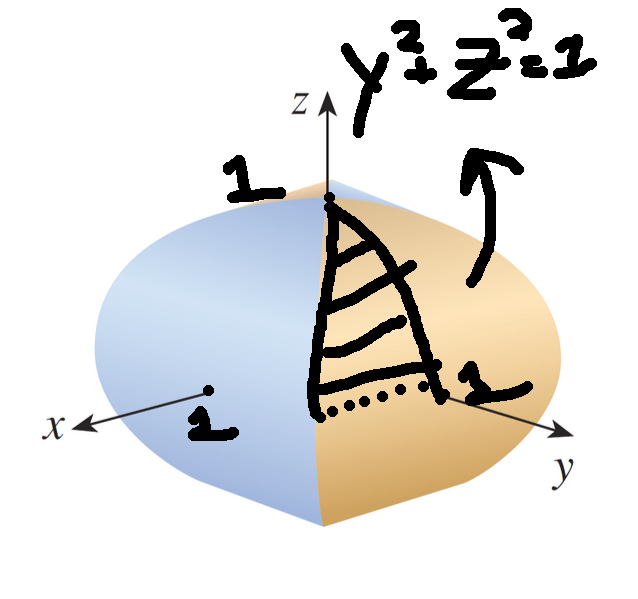
\includegraphics[width=0.5\textwidth]{calculus/W4/img/pr1}
  \caption{Subregion}
\end{figure}


Therefore, the volume can be evaluated as follows:
\begin{equation*}
  A = 16 \int_0^1 \int_x^1 \sqrt{1 + (\frac{\partial z}{\partial y})^2} dy dx, z(y) = \sqrt{1 - y^2}
\end{equation*}
\begin{equation*}
  = 16 \int_0^1 \int_x^1 \sqrt{1 + \frac{y^2}{1-y^2}} dy dx = 16 \int_0^1 \int_x^1 \frac{dy}{\sqrt{1-y^2}} dx
\end{equation*}
\begin{equation*}
  = 16 \int_0^1 \arcsin(1) - \arcsin(x) dx = 16 \int_0^1 \frac{\pi}{2} -  \arcsin(x) dx = 16 (\frac{\pi x}{2} - x\arcsin(x) - \sqrt{1-x^2})_0^1 = 16 \cdot 1
\end{equation*}

Answer: 16.

\section{ Problem 2 } 

\textbf{a)} A circle with radius R is defined on $D = \{(x, y) | -R \le x \le R\ \wedge -\sqrt{R^2 - x^2} \le y \le \sqrt{R^2 - x^2} \}$. Thus, the area is defined by:

\begin{equation*}
  \iint_{D} dA = \int_{-R}^{R} \int_{-\sqrt{R^2-x^2}}^{\sqrt{R^2-x^2}}dydx = 2\int_{-R}^{R}\sqrt{R^2 - x^2} dx
\end{equation*}

Use substitution $u = \frac{x}{R}, du = \frac{dx}{R}$. Thus,
\begin{equation*}
  2R^2\int_{-1}^{1}\sqrt{1 - u^2} du
\end{equation*}

The following integral will be used frequently:
\begin{equation*}
  \int \sqrt{1-x^2}dx = \frac{1}{2} (\arcsin(x) + x\sqrt{1-x^2}) + constant,  \int_{-1}^{1} \sqrt{1-x^2}dx = \frac{\pi}{2}
\end{equation*}


Thus,
\begin{equation*}
  2R^2\int_{-1}^{1}\sqrt{1 - u^2} du = 2R^2\frac{1}{2}(\arcsin(1) + 1\sqrt{1-1^2} - \arcsin(-1) - (-1)\sqrt{1 - (-1)^2}) = R^2(\frac{\pi}{2} + 0 - \frac{-\pi}{2} - 0) = \pi R^2
\end{equation*}

\begin{equation*}
  V_2(R) = \pi R^2
\end{equation*}

\textbf{b)} Computations are largely similar, but the domain is a 3D volume: $$D = \{(x, y, z) | -R \le x \le R \wedge -\sqrt{R^2 - x^2} \le y \le \sqrt{R^2 - x^2} \wedge -\sqrt{R^2 - x^2 - y^2} \le z \le \sqrt{R^2 - x^2 - y^2} \}$$

Thus, the volume is defined as:
\begin{equation*}
  \iiint_D dV = \int_{-R}^{R} \int_{-\sqrt{R^2 - x^2}}^{\sqrt{R^2 - x^2}} \int_{-\sqrt{R^2 - x^2 - y^2}}^{\sqrt{R^2 - x^2 - y^2}}dzdydx = 2 \int_{-R}^{R} \int_{-\sqrt{R^2 - x^2}}^{\sqrt{R^2 - x^2}} \sqrt{R^2-x^2-y^2} dydx   
\end{equation*}

Calculate iterated integrals separately:

\begin{equation*}
  \int_{-\sqrt{R^2 - x^2}}^{\sqrt{R^2 - x^2}} \sqrt{R^2-x^2-y^2} dy = \sqrt{R^2 - x^2} \int_{-\sqrt{R^2 - x^2}}^{\sqrt{R^2 - x^2}} \sqrt{1 - (\frac{y}{\sqrt{R^2 - x^2}})^2 } dy
\end{equation*} 

Use substituion $u = \frac{y}{\sqrt{R^2-x^2}}$. Thusly,

\begin{equation*}
  = (R^2-x^2) \int_{-1}^{1} \sqrt{1 - u^2} du = \frac{(R^2 - x^2)\pi}{2}
\end{equation*} 

Calculate the outer integral:
\begin{equation*}
  2 \int_{-R}^{R} \frac{(R^2 - x^2)\pi}{2} dx = \pi [R^2x - x^3/3]_{-R}^{R} = \pi [ R^3 - R^3 / 3 + R^3 - R^3 / 3 ] \Rightarrow V_3(R) =  \frac{4}{3}\pi R^3
\end{equation*}

\textbf{c)} The process is totally identical, therefore I provide only mathematical steps:

\begin{equation*}
\iiiint_{D} dW = \int_{-R}^{R} \int_{-\sqrt{R^2 - x^2}}^{\sqrt{R^2 - x^2}} \int_{-\sqrt{R^2 - x^2 - y^2}}^{\sqrt{R^2 - x^2 - y^2}}\int_{-\sqrt{R^2 - x^2 - y^2 - z^2}}^{\sqrt{R^2 - x^2 - y^2 - z^2}}dwdzdydx
\end{equation*}

\begin{equation*}
  = 2 \int_{-R}^{R} \int_{-\sqrt{R^2 - x^2}}^{\sqrt{R^2 - x^2}} \int_{-\sqrt{R^2 - x^2 - y^2}}^{\sqrt{R^2 - x^2 - y^2}} \sqrt{R^2-x^2-y^2-z^2} dzdydx
\end{equation*}

First integral.
\begin{equation*}
  \int_{-\sqrt{R^2 - x^2 - y^2}}^{\sqrt{R^2 - x^2 - y^2}} \sqrt{R^2-x^2-y^2-z^2} dz = (R^2-x^2-y^2) \int_{-1}^{1} \sqrt{1-u^2} du = \frac{\pi (R^2-x^2-y^2)}{2}
\end{equation*}

Substitute this back in the formula for the hypervolume:
\begin{equation*}
  \iiiint_{D} dW = \pi \int_{-R}^{R} \int_{-\sqrt{R^2 - x^2}}^{\sqrt{R^2 - x^2}} (R^2 - x^2 - y^2) dydx
\end{equation*}

Second integral.
\begin{equation*}
  \int_{-\sqrt{R^2 - x^2}}^{\sqrt{R^2 - x^2}} (R^2 - x^2 - y^2) dy = [y(R^2-x^2) - \frac{y^3}{3}]_{-\sqrt{R^2 - x^2}}^{\sqrt{R^2 - x^2}} = 2(R^2-x^2)^{3/2} - \frac{2}{3} (R^2-x^2)^{3/2}
\end{equation*}

\begin{equation*}
  = \frac{4}{3} (R^2-x^2)^{3/2} \Rightarrow V_4(R) = \frac{4\pi}{3}\int_{-R}^{R} (R^2 - x^2)^{3/2} dx
\end{equation*}

Use substitution $u = x/R$.
\begin{equation*}
  \frac{4\pi}{3} R^3 \int_{-R}^{R} (1 - \frac{x^2}{R^2})^{3/2} dx = \frac{4\pi}{3}R^4 \int_{-1}^{1} (1-u^2)^{3/2} dx
\end{equation*}

Substitute $u = sin\theta, du = cos\theta d\theta$

\begin{equation*}
  \int_{-1}^{1} (1-u^2)^{3/2} du = \int_{-\frac{\pi}{2}}^{\frac{\pi}{2}} \cos^4{\theta} d\theta = ... = \frac{3\pi}{8}
\end{equation*}

Therefore, $V_4(R) = \frac{4\pi}{3} R^4 \frac{3\pi}{8} = \frac{\pi^2}{2} R^4 $

\textbf{d)} In order to solve this problem, I use hyperspherical coordinates that I was not able to understand and imagine but it is not necessary for this problem because of hyperspherical symmetry. I define $d\Omega_{n}$ to include all angular differentials in spherical coordinates. Besides, I use \textbf{gamma function $\Gamma(n)$}, defined as $\int_{0}^{\infty} t^{n-1}e^{-t} dt$.

Thus, the volume of a n-sphere is defined as follows:
\begin{equation*}
  {\int \cdots \int}_{||\mathbf{x}|| \le R} d^n\mathbf{x} = \int_{0}^{R} \int_{\Omega_{n-1}} r^{n-1}drd\Omega_{n-1}
\end{equation*}

$d\Omega_{n-1}$ integral has bounds from 0 to $\pi$ for one angle, and for all others it is from 0 to $2\pi$. Use Fubini's theorem to separate integrals, and define $A_{n-1} = \int_{\Omega_{n-1}} d\Omega_{n-1}$:
\begin{equation} \label{eq:hypervolume}
   {\int \cdots \int}_{||\mathbf{x}|| \le R} d^n\mathbf{x}  = A_{n-1}\frac{R^n}{n}
\end{equation}

We can calculate $A_{n-1}$ by integrating $f(x) = e^{-||\mathbf{x}||^2}$ over $\mathbb{R}^n$. For this, evaluate the following integral:
\begin{equation*}
  \int_{0}^{\infty}t^{n-1}e^{-t^2}dt = \frac{1}{2}\int_{0}^{\infty} u^{\frac{n-2}{2}} e^{-u} du, u = t^2, du = 2tdt
\end{equation*}

\begin{equation*}
  \Rightarrow \int_{0}^{\infty}t^{n-1}e^{-t^2}dt = \frac{1}{2} \Gamma(\frac{n}{2})
\end{equation*}

Besides, it is a well-known integral: $\int_{-\infty}^{\infty} e^{-x^2} dx = \sqrt{\pi}$

Now, we put all the pieces together and find $A_{n-1}$:
\begin{equation*}
   \int_0^\infty \cdots \int_0^\infty e^{-||\mathbf{x}||^2}  d^n\mathbf{x} = A_{n-1} \int_0^\infty e^{-r^2} r^{n-1} dr = A_{n-1} \frac{1}{2} \Gamma(\frac{n}{2})
 \end{equation*}

 \begin{equation*}
   \int_0^\infty \cdots \int_0^\infty e^{-||\mathbf{x}||^2}  d^n\mathbf{x} = \int_0^\infty e^{-x_1^2} dx_1 \cdots \int_0^\infty e^{-x_n^2} dx_n = \pi^{n/2}
 \end{equation*}

 Comparing, we have:
 \begin{equation*}
   A_{n-1} = \frac{2\pi^{n/2}}{\Gamma(\frac{n}{2})}
 \end{equation*}

 Therefore, after substituting it back into Eq.~\eqref{eq:hypervolume}, we obtain the final formulae:
 \begin{equation*}
   V_n(R) = {\int \cdots \int}_{||\mathbf{x}|| \le R} d^n\mathbf{x}  = A_{n-1}\frac{R^n}{n} =  \frac{2\pi^{n/2}}{\Gamma(\frac{n}{2})} \frac{R^n}{n} = \frac{\pi^{n/2}}{\Gamma(\frac{n}{2})} \frac{R^n}{\frac{n}{2}}
 \end{equation*}

Thus, $V_n(R) = \frac{\pi^{n/2} R^n}{\Gamma(1 + \frac{n}{2})}$.

\textbf{e)} From computer science, I know that $O(n!) > O(c^n)$. Since for integers $\Gamma(n)$ is practically a factorial, $V_n(1)$ indeed goes to $0$ as $n \rightarrow \infty$. However, I was not able to come up with a mathematical proof.

\textbf{f)} I was not able to find the derivative of the volume with repsect to $n$.

\section{ Problem H3 }

\textbf{a)} Since we integrate over $[0,t] \times [0,t], t \rightarrow 1^-$, we can expand using geometric series:
\begin{equation*}
  \lim_{t \rightarrow 1^-}\int_0^t \int_0^t \frac{1}{1-xy} dxdy = \lim_{t \rightarrow 1^-} \int_0^t \int_0^t \sum_{i=0}^\infty x^iy^i dxdy = \lim_{t \rightarrow 1^-} \int_0^t \sum_{i=0}^\infty y^i \int_0^t x^i dxdy = \lim_{t \rightarrow 1^-} \int_0^t \sum_{i=0}^\infty y^i [\frac{x^{i+1}}{i+1}]_0^t dy
\end{equation*}
Similarly for the dx-integral:
\begin{equation*}
  = \lim_{t \rightarrow 1^-} \int_0^t \sum_{i=0}^\infty \frac{t^{i+1}y^i}{i+1} dy = \lim_{t \rightarrow 1^-} \sum_{i=0}^{\infty} \frac{t^{i+1}}{i+1} [\frac{y^{i+1}}{i+1}]_0^t = \lim_{t \rightarrow 1^-} \sum_{i=0}^\infty \frac{t^{2(i+1)}}{(i+1)^2} = \sum_{i=0}^\infty \frac{1}{(i+1)^2} 
\end{equation*}
Make substitution $n = i+1$. So, $i=0$ changes to $n=0+1=1$, and $\infty$ changes to $\infty+1=\infty$. Thus,
\begin{equation*}
  \int_0^1 \int_0^1 \frac{1}{1-xy} dxdy = \sum_{n=1}^\infty \frac{1}{n^2}
\end{equation*}

\textbf{b)} To transform coordinates $(x,y)$ to $(u, v)$, we need to transform the boundary and the area element.

\begin{equation*}
  \det (\mathbf{J}) = \begin{vmatrix}
x_u & x_v \\
y_u & y_v 
  \end{vmatrix} = \begin{vmatrix}
    1/\sqrt{2} & -1/\sqrt{2} \\
    1/\sqrt{2} & 1/\sqrt{2}
    \end{vmatrix} = 1
\end{equation*}

Thus, the area element is $dxdy = dudv$. Now, transform boundaries. 

\begin{equation*}
  x = 0 \Rightarrow u = v \mbox{ and } x = 1 \Rightarrow u = v + \sqrt{2}
\end{equation*}
\begin{equation*}
  y = 0 \Rightarrow u = -v \mbox{ and } y = 1 \Rightarrow u = \sqrt{2} - v
\end{equation*}

\begin{figure}[H]
  \centering
  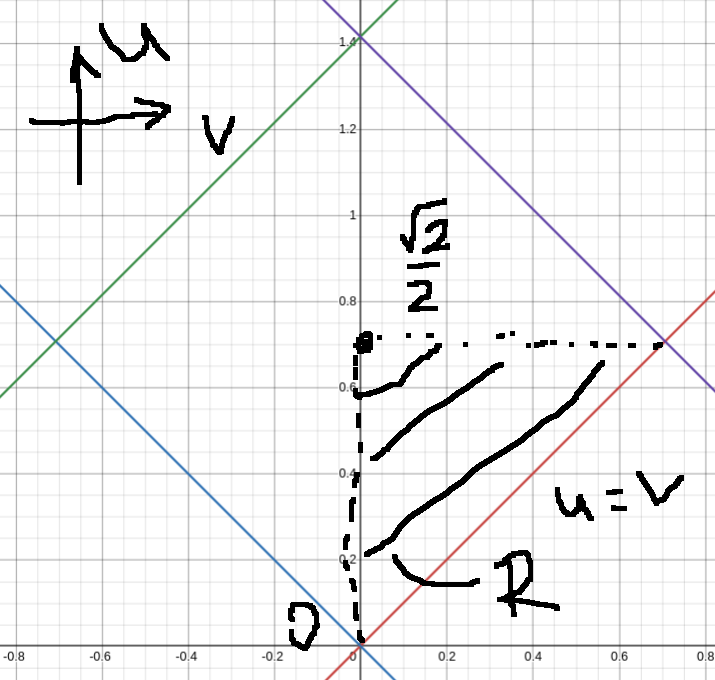
\includegraphics[width=0.5\textwidth]{calculus/W4/img/rh}
  \caption{Transformed Region}
\end{figure}

Due to symmetry, we obtain:
\begin{equation*}
  \int_0^1 \int_0^1 \frac{1}{1-xy} dxdy = 2 \int_{u=0}^{\sqrt{2}/2} \int_{v=0}^{u} \frac{1}{1 - \frac{(u+v)(u-v)}{2}} dvdu + 2\int_{u=\sqrt{2}/2}^{\sqrt{2}} \int_{v=0}^{\sqrt{2}-u} \frac{1}{1 - \frac{(u+v)(u-v)}{2}} dvdu
\end{equation*}

\textbf{Evaluate the first term: $2 \int_{u=0}^{\sqrt{2}/2} \int_{v=0}^{u} \frac{1}{1 - \frac{(u+v)(u-v)}{2}} dvdu$}

Evaluate the inner integral.
\begin{equation*}
  \int_{v=0}^u \frac{2dv}{2-u^2+v^2} = \frac{2}{\sqrt{2-u^2}} \arctan \frac{u}{\sqrt{2-u^2}}
\end{equation*}

Evaluate outer integral.
\begin{equation*}
  2 \int_{u=0}^{\sqrt{2}/2} \frac{2}{\sqrt{2-u^2}} \arctan \frac{u}{\sqrt{2-u^2}} du = 4 \int_{u=0}^{\sqrt{2}/2} \frac{du}{\sqrt{2-u^2}} \arctan \frac{u}{\sqrt{2-u^2}} 
\end{equation*}

Use substitution $u=\sqrt{2}\sin{t}$, $du = \sqrt{2} \cos(t) dt$, $t = \arcsin(u/\sqrt{2})$.
\begin{equation*}
  4 \int_{\arcsin(0/\sqrt{2})}^{\arcsin(\frac{\sqrt{2}}{2}/\sqrt{2})} \frac{\sqrt{2}\cos(t) dt}{\sqrt{2-(\sqrt{2} \sin(t))^2}} \arctan \frac{\sqrt{2} \sin(t)}{\sqrt{2-(\sqrt{2} \sin(t))^2}} = 4 \int_{0}^{\pi/6} t dt = \frac{4 \pi^2}{36 \times 2} = \frac{\pi^2}{18} 
\end{equation*}


\textbf{Evaluate the second term: $2\int_{u=\sqrt{2}/2}^{\sqrt{2}} \int_{v=0}^{\sqrt{2}-u} \frac{1}{1 - \frac{(u+v)(u-v)}{2}} dvdu$}

Evaluate the inner integral.

\begin{equation*}
  \int_{v=0}^{\sqrt{2}-u} \frac{2}{2 - u^2 + v^2} dv =
  \frac{2}{\sqrt{2-u^2}} \arctan \frac{v}{\sqrt{2-u^2}} |_{0}^{\sqrt{2}-u} = \frac{2}{\sqrt{2-u^2}} \arctan \frac{\sqrt{2}-u}{\sqrt{2-u^2}}
\end{equation*}

Evaluate the outer integral.
\begin{equation*}
  2\int_{u=\sqrt{2}/2}^{\sqrt{2}} \frac{2}{\sqrt{2-u^2}} \arctan \frac{\sqrt{2}-u}{\sqrt{2-u^2}} du
\end{equation*}

Again, use substitution $u=\sqrt{2}\sin{t}$, $du = \sqrt{2} \cos(t) dt$, $t = \arcsin(u/\sqrt{2})$.
\begin{equation*}
  = 2\int_{\arcsin{1/2}}^{\arcsin{1}} \frac{2}{\sqrt{2 - 2\sin^2{t}}} \arctan \frac{\sqrt{2} - \sqrt{2}\sin(t)}{\sqrt{2 - 2\sin^2(t)}} \sqrt{2} \cos(t) dt =
  4 \int_{\pi/6}^{\pi/2} \frac{\cos(t)}{\cos(t)} \arctan \frac{1 - \sin(t)}{\cos(t)} dt
\end{equation*}
\begin{equation*}
  = 4 \int_{\pi/6}^{\pi/2} \arctan \frac{1-\sin(t)}{\cos(t)} dt
\end{equation*}

Perform the following trigonometric transformations:
\begin{equation*}
  \frac{1- \sin(t)}{\cos(t)} = \frac{ \sin(\pi/2) - \sin(t) }{ \sin(\pi/2 - t) } = \frac{ 2 \sin(\frac{\pi/2 - t}{2}) \cos(\frac{\pi/2 + t}{2}) }{ 2\sin{\frac{ \pi/2 - t }{2}} \cos{\frac{ \pi/2 - t }{2} } } = \frac{\cos(\pi/4 + t/2)}{\cos(\pi/4 - t/2)} = \frac{\sin(\pi/2 - \pi/4 - t/2)}{ \cos(\pi/4 - t/2) } =\frac{\sin(\pi/4 - t/2)}{ \cos(\pi/4 - t/2) } 
\end{equation*}
\begin{equation*}
  = \tan(\pi/4 - t/2)
\end{equation*}
  
Thus, evaluating the intergral, we get:
\begin{equation*}
  4 ( \frac{\pi t}{4} - \frac{t^2}{4} )_{\pi/6}^{\pi/2} = \pi t - t^2 |_{\pi/6}^{\pi/2} = \frac{\pi^2}{9}
\end{equation*}

Therefore,
\begin{equation*}
  \int_0^1 \int_0^1 \frac{1}{1-xy} dxdy = \frac{\pi^2}{9} + \frac{\pi^2}{18} = \frac{\pi^2}{6} 
\end{equation*}

\textbf{c)}

\begin{equation*}
  \int_0^1 \int_0^1 \int_0^1 \frac{1}{1-xyz} dxdydz = \lim_{t \rightarrow 1^-} \int_0^t \int_0^t \int_0^t \frac{1}{1-xyz} dxdydz = \lim_{t \rightarrow 1^-} \int_0^t \int_0^t \int_0^t \sum_{i=0}^{\infty} x^iy^iz^i dxdydz
\end{equation*}

\begin{equation*}
  = \lim_{t \rightarrow 1^-} \int_0^t \int_0^t \sum_{i=0}^{\infty} y^iz^i dydz \int_0^t x^i dx = \lim_{t \rightarrow 1^-} \int_0^t \int_0^t \sum_{i=0}^{\infty} y^iz^i \frac{t^{i+1}}{i+1} dydz = ... = \lim_{t \rightarrow 1^-} \sum_{i=0}^{\infty} \frac{t^{3(i+1)}}{(i+1)^3} = \sum_{i=0}^{\infty} \lim_{t \rightarrow 1^-} \frac{t^{3(i+1)}}{(i+1)^3}
\end{equation*}

\begin{equation*}
  = \sum_{i=0}^\infty \frac{1}{(i+1)^3} = \sum_{n=1}^{\infty} \frac{1}{n^3}
\end{equation*}

\section{ Problem H4 }
To go from Cartesian coordinates to spherical, we have:
\begin{equation*}
  \rho = \sqrt{x^2 + y^2 + z^2},
  \theta = \arccos(\frac{z}{\rho}),
  \phi = \arctan(\frac{y}{x})
\end{equation*}

To derive the laplacian in spherical coordinates, we need $\rho_i, \rho_{ii}, \theta_i, \theta_{ii}, \phi_i, \phi_{ii}$, where $i \in \{x, y, z\}$. Later, I provide the table of all the derivatives and derive only $\theta_x$ in this paper. Otherwise, this paper will be too bulky.

\begin{equation*}
  \theta_x = -\frac{1}{\sqrt{1 - \frac{z^2}{\rho^2}}} \frac{\partial (z/\rho)}{\partial x} = -\frac{1}{\sqrt{1 - \frac{z^2}{\rho^2}}} (-z) \frac{1}{\rho^2} \frac{\partial \rho}{\partial x} = \frac{ xz }{ \rho^3 \sqrt{1 - \frac{z^2}{\rho^2}} } = \frac{xz}{\rho^2 \sqrt{\rho^2 - z^2}} 
\end{equation*}

Below is the table of all the partial derivatives.

\begin{table}[h!]
\centering
\renewcommand{\arraystretch}{1.5} % Adjust row height
\setlength{\tabcolsep}{10pt} % Adjust column spacing
\begin{tabular}{|c|c|c|c|}
\hline
\textbf{Partial Derivative} & \textbf{$\rho$} & \textbf{$\theta$} & \textbf{$\phi$} \\
\hline
$x$ & $\frac{x}{\rho}$ & $\frac{xz}{\rho^2 \sqrt{\rho^2 - z^2}}$ & $-\frac{y}{x^2 + y^2}$ \\
\hline
$xx$ & $\frac{\rho^2 - x^2}{\rho^3}$ & $\frac{z}{\rho^2 \sqrt{\rho^2 - z^2}} - \frac{3x^2z}{\rho^4 \sqrt{\rho^2 - z^2}} - \frac{x^2z^3}{\rho^4(\rho^2 - z^2)^{3/2}}$ & $\frac{2xy}{(x^2 + y^2)^2}$ \\
\hline
$y$ & $\frac{y}{\rho}$ & $\frac{yz}{\rho^2 \sqrt{\rho^2 - z^2}}$ & $\frac{x}{x^2 + y^2}$ \\
\hline
$yy$ & $\frac{\rho^2 - y^2}{\rho^3}$ & $\frac{z}{\rho^2 \sqrt{\rho^2 - z^2}} - \frac{3y^2z}{\rho^4 \sqrt{\rho^2 - z^2}} - \frac{y^2z^3}{\rho^4(\rho^2 - z^2)^{3/2}}$ & $-\frac{2xy}{(x^2 + y^2)^2}$ \\
\hline
$z$ & $\frac{z}{\rho}$ & $\frac{z^2 - \rho^2}{\rho^2 \sqrt{\rho^2 - z^2}}$ & $0$ \\
\hline
$zz$ & $\frac{\rho^2 - z^2}{\rho^3}$ & $\frac{2z}{\rho^4} \sqrt{\rho^2 - z^2}$ & $0$ \\
\hline
\end{tabular}
\caption{Partial derivatives of spherical coordinates.}
\label{tab:partials}
\end{table}
  
Now, find $u_x$ and $u_{xx}$.
\begin{equation*}
  u_x = u_\rho \rho_x + u_\theta \theta_x + u_\phi \phi_x
\end{equation*}
\begin{equation*}
  u_{xx} = \partial_x (u_\rho \rho_x) + \partial_x (u_\theta \theta_x) + \partial_x (u_\phi \phi_x)
\end{equation*}
\begin{equation*}
  \partial_x (u_\rho \rho_x) = u_{\rho x}\rho_x + u_\rho \rho_{xx} = ( u_{\rho \rho} \rho_x + u_{\rho \theta} \theta_x + u_{\rho \phi} \phi_x )\rho_x + u_\rho \rho_{xx}
\end{equation*}

Therefore
\begin{equation*}
  \partial_x (u_\rho \rho_x) = u_\rho \rho_{xx} + u_{\rho \rho} \rho_x^2 + u_{\rho \theta} \theta_x \rho_x + u_{\rho \phi} \phi_x \rho_x
\end{equation*}
\begin{equation*}
  \partial_x (u_\theta \theta_x) = u_\theta \theta_{xx} + u_{\theta \rho} \rho_x \theta_x + u_{\theta \theta} \theta_x^2 + u_{\theta \phi} \phi_x \theta_x
\end{equation*}
\begin{equation*}
  \partial_x (u_\phi \phi_x) = u_\phi \phi_{xx} + u_{\phi \rho} \rho_x \phi_x + u_{\phi \theta} \theta_x \phi_x + u_{\phi \phi} \phi_x^2
\end{equation*}

The same equations hold for $y$ and $z$. Combining second-order partial derivatives back into $u_{xx}$, we obtain: 
\begin{equation*}
  u_{xx} = (u_\rho \rho_{xx} + u_\theta \theta_{xx} + u_\phi \phi_{xx}) + 2( u_{\theta \rho} \rho_x \theta_x + u_{\rho \phi} \phi_x \rho_x + u_{\theta \phi} \theta_x \phi_x) + (u_{\rho \rho} \rho_x^2 + u_{\theta \theta} \theta_x^2 + u_{\phi \phi} \phi_x^2)
\end{equation*}
\begin{equation*}
  u_{yy} = (u_\rho \rho_{yy} + u_\theta \theta_{yy} + u_\phi \phi_{yy}) + 2( u_{\theta \rho} \rho_y \theta_y + u_{\rho \phi} \phi_y \rho_y + u_{\theta \phi} \theta_y \phi_y) + (u_{\rho \rho} \rho_y^2 + u_{\theta \theta} \theta_y^2 + u_{\phi \phi} \phi_y^2)
\end{equation*}
\begin{equation*}
  u_{zz} = (u_\rho \rho_{zz} + u_\theta \theta_{zz} + u_\phi \phi_{zz}) + 2( u_{\theta \rho} \rho_z \theta_z + u_{\rho \phi} \phi_z \rho_z + u_{\theta \phi} \theta_z \phi_z) + (u_{\rho \rho} \rho_z^2 + u_{\theta \theta} \theta_z^2 + u_{\phi \phi} \phi_z^2)
\end{equation*}

I wrote this in a way that the same partial derivatives of $u$ are one under the other. When adding $u_{xx}$, $u_{yy}$, $u_{zz}$, take partial derivates of $u$ out of the parenthesis, and we end up with the following pattern: $\sum u_{D} f(\rho_{D}, \theta_D,\phi_D)$, where $D$ denotes partial derivatives. Now, I compute each $f(\rho_D, \theta_D, \phi_D)$ separately. After, I plug the values back into the pattern and eventually the laplacian.

\begin{equation*}
  \rho_{xx} + \rho_{yy} + \rho_{zz} = \frac{3\rho^2 - x^2 - y^2 - z^2}{\rho^3} = \frac{2}{\rho}
\end{equation*}

\begin{equation*}
  \theta_{xx} + \theta_{yy} + \theta_{zz} = \frac{2z}{\rho^4} \sqrt{\rho^2 - z^2} + \frac{2z\rho^2(\rho^2 - z^2) - (x^2 + y^2)(3z(\rho^2 - z^2) + z^3)}{\rho^4 (\rho^2 - z^2)^{3/2}}
\end{equation*}

\begin{equation*}
  = \frac{2z}{\rho^4} \sqrt{\rho^2 - z^2} + \frac{2z\rho^4 - 2z^3\rho^2 - (\rho^2 - z^2)(3z\rho^2 - 2z^3)}{\rho^4 (\rho^2 - z^2)^{3/2}} = \frac{2z}{\rho^4} \sqrt{\rho^2 - z^2} + \frac{2z\rho^4 - 2z^3 \rho^2 - 3z\rho^4 + 2z^3\rho^2 + 3z^3\rho^2 - 2z^5}{\rho^4 (\rho^2 - z^2)^{3/2}}
\end{equation*}

\begin{equation*}
  = \frac{2z}{\rho^4} \sqrt{\rho^2 - z^2} + \frac{-z\rho^4 + 3z^3 \rho^2 - 2z^5}{\rho^4 (\rho^2 - z^2)^{3/2}} = \frac{2z(\rho^2 - z^2)^2 - z\rho^4 + 3z^3 \rho^2 - 2z^5}{\rho^4 (\rho^2 - z^2)^{3/2}} = \frac{2z(\rho^4 + z^4 - 2z^2\rho^2) - z\rho^4 + 3z^3 \rho^2 - 2z^5}{\rho^4 (\rho^2 - z^2)^{3/2}}
\end{equation*}
\begin{equation*}
  = \frac{ z }{\rho^2 \sqrt{\rho^2 - z^2}} = \frac{cos(\theta)}{\rho^2sin(\theta)}
\end{equation*}

\begin{equation*}
  \phi_{xx} + \phi_{yy} + \phi_{zz} = 0
\end{equation*}

\begin{equation*}
  \rho_x \theta_x +\rho_y \theta_y+ \rho_z \theta_z = \cdots easy_{algebra} = 0
\end{equation*}

\begin{equation*}
  \phi_x \rho_x + \phi_y \rho_y + \phi_z \rho_z = 0
\end{equation*}

\begin{equation*}
  \theta_x \phi_x + \theta_y \phi_y + \theta_z \phi_z = 0  
\end{equation*}

\begin{equation*}
  \rho_x^2 + \rho_y^2 + \rho_z^2 = 1
\end{equation*}

\begin{equation*}
  \theta_x^2 + \theta_y^2 + \theta_z^2 = \cdots = \frac{1}{\rho^2}
\end{equation*}

\begin{equation*}
  \phi_x^2 + \phi_y^2 + \phi_z^2 = \frac{(-y)^2}{(x^2+y^2)^2} + \frac{x^2}{(x^2+y^2)^2} = \frac{1}{\rho^2 - z^2} = \frac{1/\rho^2}{1 - (z/\rho)^2} = \frac{1}{\rho^2sin^2(\theta)}
\end{equation*}

Therefore,
\begin{equation*}
  \nabla^2 u = \frac{2}{\rho} u_\rho + \frac{cos(\theta)} {\rho^2sin(\theta)} u_\theta + u_{\rho \rho} + \frac{1}{\rho^2} u_{\theta \theta} + \frac{1}{\rho^2sin^2(\theta)} u_{\phi \phi}
\end{equation*}

(I think the author of the problems forgot $u_\theta$ term.)
More convenient notation:
\begin{equation*}
  \nabla^2 u = \frac{\partial^2 u}{\partial \rho^2} + \frac{2}{\rho} \frac{\partial u}{\partial \rho} + \frac{cos(\theta)}{\rho^2 sin(\theta)} \frac{\partial u}{\partial \theta} + \frac{1}{\rho^2} \frac{\partial^2 u}{\partial \theta^2} + \frac{1}{\rho^2sin^2(\theta)} \frac{\partial^2 u}{\partial \phi^2}
\end{equation*}
  
\section{ Problem H5 }

First, I go from Cartesian coordinates to spherical coordinates. Because of spherical symmetry, azimuthal angle is irrelevant and can be replaced the factor $\int_0^{2\pi} d\phi = 2\pi$. Orient $z$-axis in a way that point $\mathbf{x_1} = (x_1, y_1, z_1)$ has coordinates $(0, 0, x)$, where $x$ is the distance to the point from the origin (see figure below.) 

\begin{figure}[H]
  \centering
  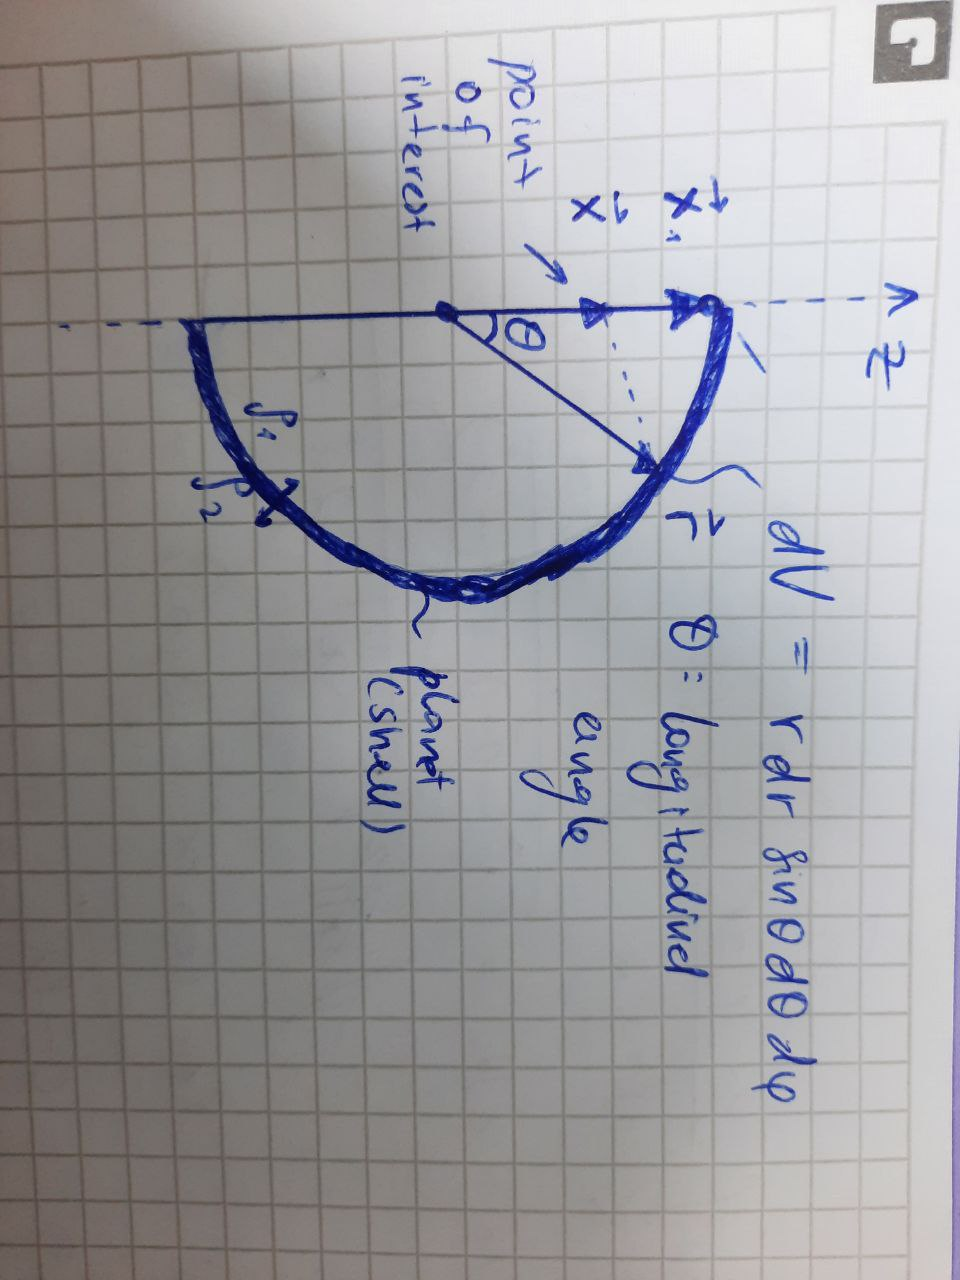
\includegraphics[width=0.5\textwidth, angle=90]{calculus/W4/img/gravity}
  \caption{Sphere}
\end{figure}

If $\omega$ denotes the region of the shell and $\mathbf{x}$ is the point of interest, we have:
\begin{equation*}
  V(\mathbf{x}) = -Gm \int_\omega \frac{\rho(\mathbf{r}) dV(\mathbf{r})}{||\mathbf{r} - \mathbf{x} ||}
\end{equation*}

The sphere is uniform $\Rightarrow \rho(\mathbf{r}) = \rho$. Besides, we can expand $||\mathbf{r} - \mathbf{x}|| = \sqrt{(\mathbf{r} - \mathbf{x}) \cdot (\mathbf{r} - \mathbf{x})} = \sqrt{ \mathbf{r}^2 + \mathbf{x}^2 - 2\mathbf{r} \cdot \mathbf{x} }$. Therefore, $||\mathbf{r} - \mathbf{x}|| = \sqrt{r^2 + x^2 - 2rx\cos(\theta)}$, where $x$ is the distance from the origin to the point of interest. Therefore, we can re-write the integral as follows:

\begin{equation*}
  V(\mathbf{x}) = -Gm2\pi\rho \int_{\rho_1}^{\rho_2} \int_0^\pi \frac{r^2\sin(\theta)d\theta dr}{\sqrt{r^2+x^2 - 2rx\cos(\theta)}}
\end{equation*}

Evaluate the inner integral by substituting $u = r^2 + x^2 - 2rx\cos(\theta)$ and $du = 2rx\sin(\theta) d\theta$:
\begin{equation*}
  \int_0^\pi \frac{r^2\sin(\theta)d\theta}{\sqrt{r^2+x^2 - 2rx\cos(\theta)}} = \frac{r}{2x} \int_{r^2+x^2-2rx}^{r^2+x^2+2rx} \frac{du}{\sqrt{u}} = \frac{r}{x} [\sqrt{u}]_{r^2+x^2-2rx}^{r^2+x^2+2rx} = r\frac{\sqrt{r^2+x^2+2rx} - \sqrt{r^2+x^2-2rx}}{x}
\end{equation*}

\begin{equation*}
  x < \rho_1 < r \Rightarrow r\frac{\sqrt{r^2+x^2+2rx} - \sqrt{r^2+x^2-2rx}}{x} = \frac{(r+x) - (r - x)}{x} = \frac{2x}{x} = 2r
\end{equation*}

Evaluate outer integral:
\begin{equation*}
  \int_{\rho_1}^{\rho_2} 2r dr = \rho_2^2 - \rho_1^2
\end{equation*}

Thus,
\begin{equation*}
  V(\mathbf{x}) = -2Gm\pi \rho (\rho_2^2 - \rho_1^2)
\end{equation*}

Dimensional analysis does indeed yield $Joules$ for $V(\mathbf{x})$.



  
\end{document}
